\chapter{Introduction}
\label{introduction}

Currently, many exascale problems are striving for more computing power to be solved~\cite{Messina2017}. Thus, we always aim for more computing power which can empower us to solve exascale problems. Thus we are keen on advancing the way we design transistors till quantum computers become ready. Current silicon-based technology is obeying \textit{Moore's law} since 1965 where the transistor number per integrated circuit is doubling every year~\cite{Schaller1997, Moore2006}. Throughout the years since Moore's law, the technology has been advancing a lot with more and more transistors double on the same chip year after year. 

Miniaturising and down-scaling electronic devices lead to increasing the number of transistors per chip and thus raising the overall computing power of the chip~\cite{Thiele2017}. Thus, the physical characteristics of such computing devices are the controlling factors of the resultant computing frequencies and its functionality. Alternative channel materials like graphene and other 2D materials can ideally serve for this purpose. Those candidate substitutive materials are having extraordinary nanoscale electronic properties, which in turn are capable of delivering a significant boost in computing properties. Such technology acceleration can shape a new era of post-silicon industry~\cite{Schwierz2010, Geim2007, Taghioskoui2009, Schwierz2011, Kim2011, Schwierz2013}. 

Six years before Moore's law, Richard Feynman has pointed out to the possibility of achieving exceptional results when manipulating atoms. Feynman stated that during his notable talk, entitled \textit{There is plenty of Room at the Bottom}~\cite{Feynman1960}. He said '\textit{I can't see exactly what would happen, but I can hardly doubt that when we have some control of the arrangement of things on a small scale, we will get an enormously greater range of possible properties that substances can have, and of different things that we can do.}'. Since then, researchers have been investigating the atomic-level properties of different materials, exfoliating, integrating and simulating it. Graphene is an excellent example of such development. Inaugurated as Novoselov et al.~\cite{Novoselov2004} successfully exfoliated graphite layers in 2004 achieving a breakthrough towards atomic manipulation to which Feynman pointed. 

Nowadays, computing needs are not only limited to traditional computers we grow up with but are widespread to include quite a broad pool of devices ranging from laptops, tablets, smartphones, smartwatches, glasses, implantable body electronics and other useful daily usable applications. Those devices have dozens of functionalities depending on the combined usage of different integrated devices on their chips: accelerometers, gyroscopes, communication units, sensors, gyroscopes and others. The urge to advance and maximise the functionalities and hence the resultant properties of such devices has shaped what is known as \textit{more than Moore} paradigm. 

While Gordon Moore expected the evolution of device scaling throughout the years, the idea beyond the \textit{more than Moore} depends on developing applications that solve the optimisation puzzle of both achieving high diversification of functionality while miniaturising the devices year after year. Fig. \ref{fig:moore} shows an overview of this law. In detail, this law enables more features by achieving diversification through utilisation of different devices with different functions such as analogue, radio frequency, passives, high-voltage power, sensors and actuators, and biochips. Incorporating various packages containing the systems achieves diversity, in other words, it is called system-in-package (SiP). 

\begin{figure}
    \centering
    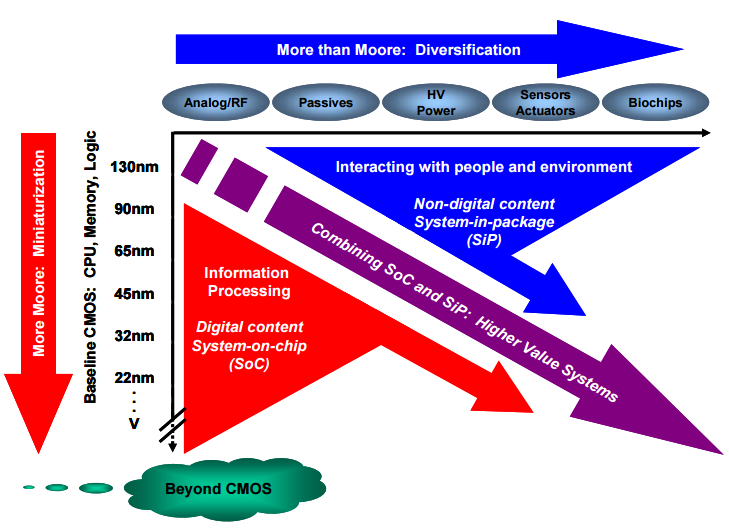
\includegraphics[width=\textwidth]{Figs/MoreThanMoore.png}
    \caption{\textit{More than Moore}. From ITRS~\cite{Arden2010}}
    \label{fig:moore}
\end{figure}

Meanwhile, those multiple components are evolving through time satisfying \textit{Moore's law} and getting miniaturised in a way that enables integrating various functionalities on the same chip, in which is called system-on-chip (SoC). Optimising both trends can achieve hatching new out-of-the-box solutions. Integrating such bulky diverse functionality devices can be achieved via exploring new ways of designing our computing units while being miniaturised. Such new directions employ on a bottom-up approach pointed by Feynman decades ago. Consequently, examining new trends in transistor material design, revolutionising the semiconductor field, becomes a necessity for enabling a combination of SiP and SoC for building higher value systems~\cite{Lemme2012}. As we have pointed above, candidate materials as graphene and other similar 2D promising materials can boost the electronic design within the more than Moore paradigm~\cite{Fiori2014nature, Fiori2015}.

After Novoselov's~\cite{Novoselov2004} effort on 2004, graphene research shed light upon potential applications due to its extraordinary properties. Specifically, a large pool of research has focused on integrating graphene in sensors~\cite{Lee2008, Geim2009, Smith2015, Smith2017}, supercapacitors~\cite{Liu2010, Yoo2011, Brownson2012}, biosensors~\cite{Shao2010, He2010}, radio frequency devices~\cite{Moon2009, Koswatta2011}, spintronics~\cite{Han2014} and photodetectors~\cite{Mueller2010, Lemme2011}. Such outstanding proven characteristics made graphene a hot topic for scientific research for the ultimate purpose of engagement within a diverse number of applications. 
%
%
\section{Research contribution}
In this work, we aim for the ultimate goal of examining graphene as a gas sensor theoretically; we elucidate the electronic structure studies of pristine single and double layered graphene residing on top of different substrates types as well as the adsorbates-graphene interactions and the influence coming from the substrate surface defects. We specifically investigate the interplay between the substrate common surface defects and the adsorbed water and carbon dioxide molecules on top of graphene sheets. We performed the studies via means of a first-principle \textit{ab-initio} method within dispersion corrected studies.
%
%
\section{Thesis organisation}
The thesis is compiled into seven chapters, detailed as the following:
\begin{itemize}
\item \textbf{Chapter 1} provides a background of the current trends in technology and motivation for this thesis work.
\item \textbf{Chapter 2} provides some insights on graphene theory.
\item \textbf{Chapter 3} focuses on the sensing mechanism of graphene and literature comparison with other materials in use.
\item \textbf{Chapter 4} presents some theoretical overview covering the method.
\item \textbf{Chapter 5} gives some insights on the used calculational parameters with an overview and recommendations of some technicalities related to the programs and method in use.
\item \textbf{Chapter 6} summarises the results of the related thesis's manuscripts.
\item \textbf{Chapter 7} outlooks the thesis work with some insights on some futuristic disciples and paths to go through.
\end{itemize}
\endinput
